\begin{figure}[h!]
	\centering
	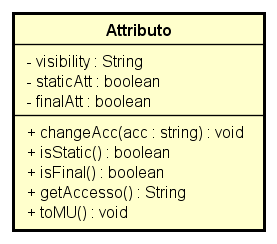
\includegraphics[scale=0.8]{res/sections/SpecificaFrontEnd/Services/Disegnetti/attributo.png}
	\caption{Diagramma della classe Attributo}
\end{figure}

\begin{itemize}
	\item \textbf{Descrizione:}\\
	
	\item \textbf{Utilizzo:}\\
	
	\item \textbf{Attributi:}
		\begin{itemize}
			\item \emph{-visibility: string}\\
			
			\item \emph{-staticAtt: boolean}\\
			
			\item \emph{-finalAtt: boolean}\\
			
		\end{itemize}
	\item \textbf{Metodi:}
		\begin{itemize}
			\item \emph{+changeAcc(acc: string)}\\
    		\\
    		\textbf{Parametri:}
    		\begin{itemize}
    			\item \emph{acc: string}\\
    			
    		\end{itemize}
    		\item \emph{+isStatic()}\\
    		Ritorna true se l'attributo è statico
    		\item \emph{+isFinal()}\\
    		Ritorna true se l'attributo è final
    		\item \emph{+getAccesso()}\\
    		Ritorna la visibilità dell'attributo
    		\item \emph{+toMU()}\\
    		
    	\end{itemize}
\end{itemize}